% Préambule commun des schémas TikZ (compilés séparément par construire_figures.py)
\documentclass[tikz,border=3pt]{standalone}
\usepackage[T1]{fontenc}
\usepackage[utf8]{inputenc}
\usepackage{lmodern}
\usepackage{amsmath,amssymb}
\usepackage{bm}
\usepackage[american,siunitx,straightvoltages]{circuitikz}
\usetikzlibrary{arrows.meta,positioning,calc,decorations.pathmorphing,
  decorations.markings,decorations.pathreplacing,patterns,shapes.geometric,
  shapes.misc,shapes.multipart,fit,backgrounds,3d,intersections,matrix}

\ctikzset{bipoles/length=1.1cm, amplifiers/scale=0.85, tripoles/op amp/width=1.4}

\tikzset{
  >={Latex[length=2mm,width=1.4mm]},
  every picture/.style={line width=0.6pt, font=\small},
  % schémas-blocs
  bloc/.style={draw, minimum width=1.5cm, minimum height=0.9cm, align=center,
               inner sep=3pt, fill=white},
  somme/.style={draw, circle, minimum size=4.5mm, inner sep=0pt, fill=white,
                path picture={\draw (path picture bounding box.north west)
                  -- (path picture bounding box.south east)
                  (path picture bounding box.north east)
                  -- (path picture bounding box.south west);}},
  gain/.style={draw, isosceles triangle, isosceles triangle apex angle=60,
               minimum size=8mm, inner sep=1pt, fill=white},
  bruit/.style={draw, circle, minimum size=4.5mm, inner sep=0pt, fill=white,
                path picture={\node at (path picture bounding box.center)
                  {\scriptsize$\ast$};}},
  cadre/.style={draw, dashed, rounded corners=1pt},
  cadrept/.style={draw, dash dot, rounded corners=1pt},
  fleche/.style={->},
  % mécanique
  bati/.style={pattern=north east lines, draw=none},
  ressort/.style={decorate, decoration={coil, aspect=0.4, segment length=2.2mm,
                  amplitude=2mm, pre length=2mm, post length=2mm}},
  zigzag/.style={decorate, decoration={zigzag, segment length=2mm,
                  amplitude=1.6mm, pre length=2mm, post length=2mm}},
  pivot/.style={draw, circle, fill=white, minimum size=2.2mm, inner sep=0pt},
  masse/.style={draw, fill=gray!25, minimum width=1.4cm, minimum height=0.8cm},
  cote/.style={<->, line width=0.4pt},
  axe/.style={->, line width=0.6pt},
  trait mixte/.style={dash dot, line width=0.4pt},
}

% Encastrement / bâti hachuré : \bati{(x1,y1)}{(x2,y2)} trace une ligne et ses hachures dessous
\newcommand{\bati}[3][0.18]{%
  \fill[pattern=north east lines] #2 rectangle ($#3+(0,-#1)$);
  \draw[line width=0.8pt] #2 -- #3;}

% Transducteur (deux cercles entrelacés) : \pic (t) at (x,y) {transducteur};  -> (t-o) entrée, (t-e) sortie
\tikzset{
  transducteur/.pic={\draw (-0.13,0) circle (0.24); \draw (0.13,0) circle (0.24);
    \coordinate (-o) at (-0.37,0); \coordinate (-e) at (0.37,0);
    \coordinate (-n) at (0,0.24); \coordinate (-s) at (0,-0.24);},
  bobine/.style={decorate, decoration={coil, aspect=0.7, segment length=1.4mm,
                 amplitude=1.6mm, pre length=1mm, post length=1mm}},
  sourcebruit/.style={draw, circle, minimum size=5mm, inner sep=0pt, fill=white,
                 label={[inner sep=0pt]center:$\ast$}},
  sourcecourant/.style={draw, circle, minimum size=5mm, inner sep=0pt, fill=white,
                 label={[inner sep=0pt]center:$\circledast$}},
}

% Composants compacts (pour les petits boîtiers des schémas-blocs)
\newcommand{\resistance}[2]{% de #1 à #2 (quelconque)
  \draw #1 -- ($#1!0.22!#2$) ($#1!0.78!#2$) -- #2;
  \draw[decorate, decoration={zigzag, segment length=1.5mm, amplitude=1.1mm}]
    ($#1!0.22!#2$) -- ($#1!0.78!#2$);}
\newcommand{\condensateur}[2]{% horizontal de #1 à #2
  \draw #1 -- ($($#1!0.5!#2$)+(-0.05,0)$) ($($#1!0.5!#2$)+(0.05,0)$) -- #2;
  \draw[line width=1pt] ($($#1!0.5!#2$)+(-0.05,0.14)$) -- ($($#1!0.5!#2$)+(-0.05,-0.14)$)
                        ($($#1!0.5!#2$)+(0.05,0.14)$) -- ($($#1!0.5!#2$)+(0.05,-0.14)$);}
% R // C horizontal : \RparC{(x,y)}{longueur}{écart}  (centre, longueur totale, écart vertical)
\newcommand{\RparC}[3]{%
  \coordinate (rcA) at ($#1+(-#2/2,0)$); \coordinate (rcB) at ($#1+(#2/2,0)$);
  \draw (rcA) -- ++(0.15,0) coordinate (rcA1) (rcB) -- ++(-0.15,0) coordinate (rcB1);
  \draw (rcA1) -- ++(0,#3/2) (rcA1) -- ++(0,-#3/2) (rcB1) -- ++(0,#3/2) (rcB1) -- ++(0,-#3/2);
  \resistance{($(rcA1)+(0,#3/2)$)}{($(rcB1)+(0,#3/2)$)}
  \condensateur{($(rcA1)+(0,-#3/2)$)}{($(rcB1)+(0,-#3/2)$)}}

\begin{document}
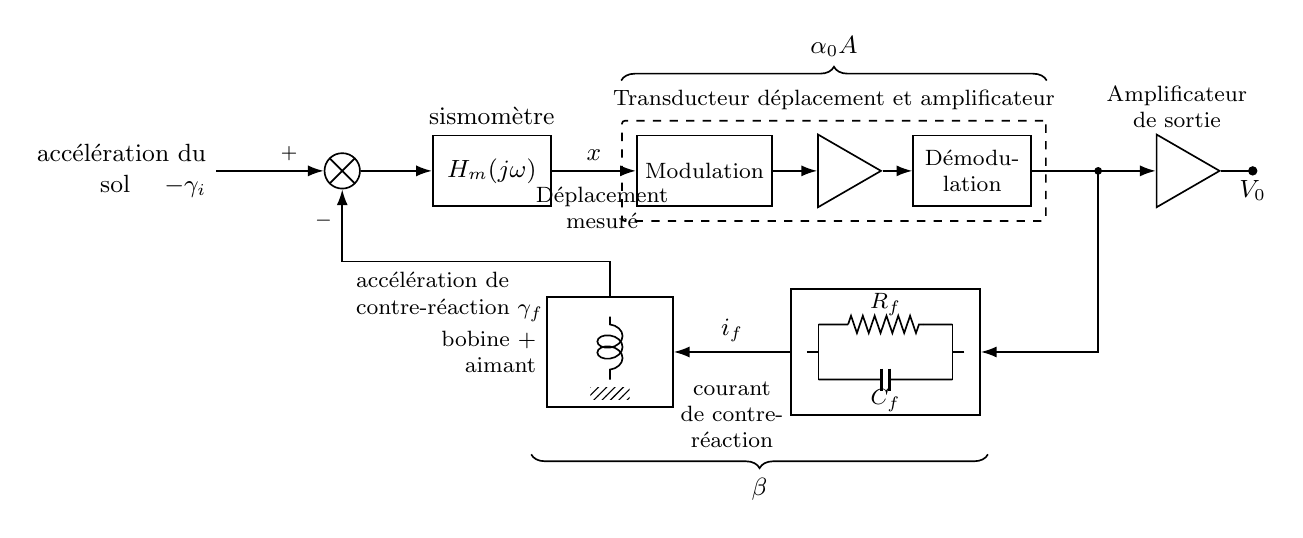
\begin{tikzpicture}[font=\small]
  \node[somme] (s) at (0,0) {};
  \node[bloc] (h) at (1.9,0) {$H_m(j\omega)$};
  \node[above] at (h.north) {sismomètre};
  \node[bloc, font=\footnotesize] (mod) at (4.6,0) {Modulation};
  \node[gain] (amp) at (6.3,0) {};
  \node[bloc, font=\footnotesize, align=center] (dem) at (8.0,0) {Démodu-\\lation};
  \node[cadre, fit=(mod) (dem), inner sep=5pt] (td) {};
  \node[above, font=\footnotesize] at (td.north) {Transducteur déplacement et amplificateur};
  \draw[decorate, decoration={brace, amplitude=5pt}] ([yshift=5mm]td.north west) -- ([yshift=5mm]td.north east)
     node[midway, above=5pt] {$\alpha_0 A$};
  \node[gain] (sor) at (10.6,0) {};
  \node[above=1mm, align=center, font=\footnotesize] at (sor.north) {Amplificateur\\de sortie};
  \draw[->] (-1.6,0) node[left, align=right] {accélération du\\sol \quad $-\gamma_i$} -- (s) node[above left, pos=0.85] {\scriptsize$+$};
  \draw[->] (s) -- (h);
  \draw[->] (h) -- node[above] {$x$} (mod);
  \node[below, align=center, font=\footnotesize] at (3.3,-0.08) {Déplacement\\mesuré};
  \draw[->] (mod) -- (amp); \draw[->] (amp) -- (dem); \draw[->] (dem) -- (sor);
  \draw (sor.east) -- ++(0.4,0) node[circle, fill, inner sep=1.2pt] {} node[below] {$V_0$};
  % contre-réaction
  \coordinate (n) at (9.6,0); \fill (n) circle (1.4pt);
  \node[bloc, minimum width=2.4cm, minimum height=1.6cm] (rc) at (6.9,-2.3) {};
  \RparC{(6.9,-2.3)}{2.0}{0.7}
  \node[font=\footnotesize] at (6.9,-1.7) {$R_f$};
  \node[font=\footnotesize] at (6.9,-2.92) {$C_f$};
  \node[bloc, minimum width=1.6cm, minimum height=1.4cm] (bob) at (3.4,-2.3) {};
  \draw[bobine] (3.4,-1.85) -- (3.4,-2.65);
  \fill[pattern=north east lines] (3.15,-2.75) rectangle (3.65,-2.9);
  \node[left, align=right, font=\footnotesize] at (bob.west) {bobine +\\aimant};
  \draw[->] (n) |- (rc.east);
  \draw[->] (rc.west) -- node[above] {$i_f$} (bob.east);
  \node[below, align=center, font=\footnotesize] at (4.95,-2.55) {courant\\de contre-\\réaction};
  \draw[->] (bob.north) |- (0,-1.15) -- (s.south) node[below left, pos=0.8] {\scriptsize$-$};
  \node[align=left, anchor=west, font=\footnotesize] at (0.05,-1.6) {accélération de\\contre-réaction $\gamma_f$};
  \draw[decorate, decoration={brace, amplitude=5pt, mirror}] (2.4,-3.6) -- (8.2,-3.6) node[midway, below=5pt] {$\beta$};
\end{tikzpicture}
\end{document}
